% Use only LaTeX2e, calling the article.cls class and 12-point type.

\documentclass[12pt]{article}

% Users of the {thebibliography} environment or BibTeX should use the
% scicite.sty package, downloadable from *Science* at
% www.sciencemag.org/about/authors/prep/TeX_help/ .
% This package should properly format in-text
% reference calls and reference-list numbers.

\usepackage[sort]{scicite}
\usepackage{times}
\usepackage{graphicx}
\usepackage{lineno}
\usepackage{color}
\usepackage{multirow}

% The following parameters seem to provide a reasonable page setup.

\topmargin 0.0cm
\oddsidemargin 0.2cm
\textwidth 16.5cm 
\textheight 21cm
\footskip 1.0cm


%The next command sets up an environment for the abstract to your paper.

\newenvironment{sciabstract}{%
\begin{quote} \bf}
{\end{quote}}


% If your reference list includes text notes as well as references,
% include the following line; otherwise, comment it out.

%\renewcommand\refname{References and Notes}

% The following lines set up an environment for the last note in the
% reference list, which commonly includes acknowledgments of funding,
% help, etc.  It's intended for users of BibTeX or the {thebibliography}
% environment.  Users who are hand-coding their references at the end
% using a list environment such as {enumerate} can simply add another
% item at the end, and it will be numbered automatically.

\newcounter{lastnote}
\newenvironment{scilastnote}{%
\setcounter{lastnote}{\value{enumiv}}%
\addtocounter{lastnote}{+1}%
\begin{list}%
{\arabic{lastnote}.}
{\setlength{\leftmargin}{.3in}}
{\setlength{\labelsep}{.5em}}}
{\end{list}}


% Include your paper's title here

\title{The Spatial and Temporal Domains of Modern Ecology }%\\
%OR Ecology's Spatio-temporal Domains\\
%OR Space, Time, and Ecology \\
%OR Ecology: still a small-scale, field-based discipline} 
 
\author
{Lyndon Estes$^{\ast1, 2}$, Paul R. Elsen$^{3, 4}$, Tim Treuer$^{4}$, Labeeb Ahmed$^{5}$, \\
Kelly Caylor$^{6, 7}$, Jason Chang$^{5}$, Jonathan J. Choi$^{5}$, and Erle Ellis$^{6}$ \\
\\
\normalsize{$^{1}$Graduate School of Geography, Clark University, Worcester MA 01610, USA}\\
\normalsize{$^{2}$Woodrow Wilson School, Princeton University, Princeton, NJ 08544, USA}\\
\normalsize{$^{3}$Department of Environmental Science, Policy, and Management,}\\
\normalsize{University of California Berkeley, Berkeley, CA 94720, USA}\\
\normalsize{$^{4}$Ecology and Evolutionary Biology, Princeton University, Princeton, NJ 08544, USA}\\
\normalsize{$^{5}$Geography and Environmental Systems, University of Maryland Baltimore County,}\\ 
\normalsize{Baltimore, MD 21250, USA}\\
\normalsize{$^{6}$Department of Geography, University of California Santa Barbara, Santa Barbara, CA 93106, USA}\\
\normalsize{$^{7}$Bren School of Environmental Science and Management,}\\
\normalsize{University of California Santa Barbara, Santa Barbara, CA 93106, USA}\\
\normalsize{$^\ast$To whom correspondence should be addressed; E-mail:  LEstes@clarku.edu.}}
% Include the date command, but leave its argument blank.

\date{}


%%%%%%%%%%%%%%%%% END OF PREAMBLE %%%%%%%%%%%%%%%%

\begin{document} 

% Double-space the manuscript.

\baselineskip24pt

% Make the title.

\maketitle 

\section*{Abstract}
\textbf{To properly understand ecological phenomena, it is necessary to observe them across a range of spatial and temporal scales. Ecologists first raised this point in the 1980s, and since then the ability to collect multi-scale observations has grown rapidly. To assess modern ecology's progress in addressing scale, we analyzed the resolution, extent, interval, and duration of observations in 348 observational studies published between 2004-2014. We found that the scale domains of observations are fairly narrow, and are collected primarily with conventional field techniques. In the spatial domain, most observations have resolutions of $\leq$1 m2 and extents of $\leq$10,000 ha. In the temporal domain, most observations were either unreplicated or of low frequency ($\geq$1 month interval), and were made over relatively short durations ($\leq$1 year). Compared to prior meta-analyses from the 1980s and early 2000s, observational durations and resolutions remain largely unchanged, but intervals have become finer and extents larger. Despite such gains, a large gulf exists between the scales at which phenomena are actually observed, and the scales those observations ostensibly represent, revealing portions of space and time not truly captured by replicates and raising concerns about observational comprehensiveness. Adding to these concerns, scales were not clearly reported in most studies, suggesting that it is a minor consideration. Journals can help mitigate this problem by implementing scale reporting standards, which can spur ecologists to more rapidly adopt new observational technologies, and thereby close key gaps in current observational domains.} 


\linenumbers
\vspace{10pt}
The scales at which ecosystems are observed play a critical role in shaping our understanding of their structure and function \cite{levin_problem_1992,chave_problem_2013,wiens_spatial_1989}.  Ecological patterns emerge from temporal and spatial domains that may be coarser or finer than the processes that shape them, which means that investigation across multiple scales is essential for understanding ecological phenomena \cite{levin_problem_1992,sandel_scale_2009}. This awareness has grown rapidly since the 1980s, accelerated by the need to understand how changes in the global climate, ocean, and land systems are affecting everything from individual populations \cite{tingley_push_2012} to entire biomes \cite{xiao_photosynthetic_2004}, while technological advances in areas such as remote sensing and genetics are making it ever-easier to quantify ecological features across a broad and increasing range of scales \cite{schneider_rise_2001, chave_problem_2013}.  

Given the growing awareness of scale, expanding data gathering capabilities, and the fact that the most comprehensive (and arguably best-known) meta-analyses \cite{tilman_ecological_1989,kareiva_spatial_1988} of ecological research scales were published nearly 30 years ago (but see \cite{porter_crop_2005,sandel_scale_2009} for more recent reviews), it is both timely and important to assess the scales of contemporary ecological investigation. To address this need, we quantified the spatial and temporal domains of empirical observations that were reported within recently (2004-2014) published ecological studies. We define domain as the distribution of observations within the spectrum of one or more scale dimensions\footnote{This definition differs slightly from Wiens' \cite{wiens_spatial_1989}, who defined ``domain of scale'' as ``a portion of the scale spectrum within which process-pattern relationships are consistent regardless of scale.''}, and empirical observations as ecological observations collected under un-controlled or non-manipulated conditions. Empirical observations are critical for developing and testing the models that explain why ecological patterns vary in time and space \cite{levin_problem_1992, tilman_ecological_1989}, therefore the spatio-temporal domains of observations provide an important indicator of the field's progress towards achieving a holistic, predictive understanding of ecosystems \cite{chave_problem_2013,levin_problem_1992}. 

Our analysis focused on two dimensions of spatial scale, resolution (grain) and extent, and two of temporal scale, interval and duration (Table 1, and see SI for full definitions). Resolution is the area of an individual spatial replicate within which a complete measurement (as opposed to a sub-sample) of the feature of interest was made. Extent is the area enclosed by the outer-most spatial replicates, or, if the system or habitat being sampled was distinct from its surrounding matrix (e.g. forest patches in grassland habitats), the summed area of sampled patches. Interval refers to the average time elapsed between individual temporal replicates. Duration measures the time elapsed between the first and last temporal replicates, or, in the case of temporally unreplicated observations, the estimated time spent collecting the observation. We also assessed observational scales within two additional dimensions, \emph{actual} extent (the summed area of spatial replicates) and \emph{actual} duration (the summed observational time of temporal replicates). We evaluated these additional dimensions to gain insight into how much the actual scales of observation (i.e. how much space and time is covered by the measurement) differ from the scales that the observations are explicitly or implicitly intended to represent. This difference may contain important information about how effectively ecological observations characterize ecological phenomena. First, an increasing gap between actual and intended observational scale inherently implies greater interpolation or extrapolation of observed measurements, raising the odds of over-leveraging data. Second (and relatedly), since natural systems are frequently complex, non-linear, and non-random \cite{levin_ecosystems_1998,pringle_spatial_2017,rietkerk_regular_2008}, a larger gap may increase the likelihood of encountering unanticipated data challenges such as censored data (\emph{sensu} \cite{efron_efficiency_1977}), as phenomena may resolve themselves in the space or time between observations. 

\begin{table}[htp]
\caption{The scale dimensions of ecological observations assessed in this meta-analysis.}
\begin{center}
\begin{tabular}{llll}
\hline
\multicolumn{2}{c}{\textbf{Component}} & \textbf{Units} & \textbf{Description} \\\hline\hline
\multirow{3}*{Spatial} & Resolution & m$^2$ & Area of an individual spatial replicate (e.g. plot) \\%\cmidrule(l){2-3}
   & Extent & ha & Area  encompassed by all spatial replicates \\
   & Actual extent & ha & Summed area of all spatial replicates\\\hline
\multirow{3}*{Temporal} & Interval & days & Time elapsed between successive temporal replicates \\
   & Duration & days & Time elapsed between first and last temporal replicates\\
   & Actual duration & days & Summed observational time of all temporal replicates\\
\hline
\end{tabular}
\end{center}
\label{default}
\end{table}%

%We extracted these scale dimensions from 379 observations that were reported in 134 papers that were published between 2004-2014 in the top 30 (based on 2012 impact factor) ecology-themed journals. 
%

Our analysis was based on a review of 348 papers randomly selected from 42,918 published between 2004-2014 in the top 30 (based on 2012 impact factor) ecology-themed journals. We extracted scale data from 378 observations of ``natural'' (i.e. non-experimentally manipulated) ecological features that were reported within 133 of the reviewed papers (plus an additional 62 that these cited as the source of observations). We excluded experiments because they tend to be of limited extent, duration, and resolution due to their higher logistical costs \cite{tilman_ecological_1989, kareiva_spatial_1988}, and would therefore likely bias our findings towards finer scales, while minimizing the impact that new observing methods (e.g. satellite imaging, wireless sensing) may have had in expanding the scales of ecological investigation \cite{turner_remote_2003,pettorelli_satellite_2014,porter_wireless_2005}. 

To account for uncertainty in the estimation of observational dimensions due to 1) unclear methodological description in the reviewed papers, and 2) observer interpretation, we conducted a resampling analysis (n=1000) in which scale values were randomly perturbed within the bounds of estimated inter-observer variation (SI). We constructed histograms for each dimension from the mean of the perturbed ensembles, and estimated 95\% confidence intervals for each histogram bin (Fig. 1). We constructed kernel density estimates from the full resampled ensemble in order to assess observational distributions within different juxtapositions of the four primary (resolution, extent, interval, duration) space-time dimensions (Fig. 2). 

\noindent \textbf{Results}\\
\noindent \textbf{\emph{Observational methods}}\\
To account for potential differences in scales related to methodology, we classified each observation according to the following broad categories, which were field methods (manual \emph{in situ} data collection), automated (\emph{in situ}) sensing, remote sensing/other geographic data (hereafter remote observations), and paleo-reconstruction approaches. Field methods were used for 80\% of observations, automated sensing for 12.4\%, remote sensing for 6.9\%, and paleo-reconstruction for less than 0.8\%. 

\noindent \textbf{\emph{Distributions within the four primary dimensions}}\\
In terms of resolution, spatial replicates for the majority (67\%) of observations (across all methods) were $<$1 m$^2$, a further 24\% were 1 m$^2$ up to 1 ha, and the remaining 9\% were $\geq$1 ha (Fig. 1A). These distributions primarily reflect those of field observations, the dominant observational methodology. Examining the distributions for each observational method (Fig. S1 in SI) shows that automated sensing and paleo-reconstruction had resolutions that were generally finer (85\% or more $<$0.1 m$^2$) than field observations (47\% $<$0.1 m$^2$), while the majority of remote observations were much coarser (70\% $>$100 m$^2$).   

The extent of 19\% of observations was $<$10 ha, 23\% covered 10-1,000 ha, 12\% 1,000-10,000 ha, 19\% 10,000-100,000 ha, 12\% 100,000-1,000,000 ha, and 15\% $>$1,000,000 ha (Fig. 1B).  As with resolution, the extent covered by automated sensing methods tended to be smaller (52\% $<$100 ha) than those of field observations (31\% $<$100 ha), while all but 4\% of remote observations covered areas $\geq$10,000 ha (as did the small number of paleo-reconstructions).  

%16 + 29 + 26 + 67 + 14 + 37 + 10

In the temporal dimensions, 37\% of observations were not repeated (Fig. 1C), 17\% were repeated at short intervals (sub-second to daily), 20\% at daily to monthly intervals, 18\% at monthly to yearly intervals, 6\% at yearly to decadal intervals, and 2\% at decadal or greater intervals. With respect to temporally replicated observation (Fig. S1 in SI), automated sensing techniques had the finest intervals (61\% $\leq$1 day; 100\% $\leq$1 year), followed by remote observation (37\% $\leq$1 day; 78\% $\leq$1 year), field observations (17\% $\leq$1 day; 86\% $\leq$1 year), and paleo-reconstructions (21\% $\leq$1 decade).   

Duration was one day or less for 31\% of sampled observations (due to lack of temporal replication), while 10\% covered one day to one month, 23\% lasted one month to one year, 27\% covered 1-10 years, and 9\% spanned a decade or more (including several paleoecological studies covering centuries to millennia; Fig. 1D). Paleo-reconstructions naturally had the longest duration (67\% $>$ 1 decade), while just $\sim$40\% of field, automated, and remote observations had durations of 1 year or longer.

\noindent \textbf{\emph{Spatial and temporal domains}}\\
Juxtaposing these observational dimensions provides further insight into the spatial and temporal domains of observations (Fig. 2). Contrasting resolution with interval reveals that the majority of temporally replicated observations (unrepeated observations were excluded because they lack interval values) had resolutions of 10 cm$^2$-1 m$^2$ and were revisited at daily to yearly intervals (Fig. 2A). A less dense, oblong concentration of observations bounded on the upper left by monthly to yearly observations at 100 m$^2$ resolution and on the lower right by near-daily to monthly observations with 1-10 ha resolution is also evident. The four observational methods occupied substantially different portions of the domain space, as indicated by the locations of their median values (and illustrated further in Fig. S2 in the SI): the median domain of field observations was between 0.1-1 m$^2$ of resolution with a monthly interval, whereas remote observations had coarser median resolutions (1000 m$^2$) but finer median intervals ($\sim$1 day). Paleo-reconstructions and automated sensing techniques were both finely resolved (medians from 10 cm$^2$ to 0.01 m$^2$), but automated approaches had hourly-daily median intervals compared to multi-decadal for paleo-reconstructions. 

%Comparing the spatial and temporal resolutions of  interval to spatial resolution of ecological observations reveals three primary regions of observational concentration (Fig. 2A), the greatest being unreplicated samples with resolutions of 100 cm$^2$ to 1 m$^2$, followed by observations of daily to monthly interval with slightly finer spatial resolutions (10 cm$^2$ to 1 m$^2$), and finally a smaller concentration of monthly to yearly measurements collected at spatial scales of 0.1-10 ha.  

Comparing the interval and duration of temporally replicated observations showed most observations had daily to decadal intervals and durations of $\geq$1 month up to 1 decade (Fig. 2B). The orientation of this concentration shows that interval increases with duration; observations lasting one month to one year tend to have daily to monthly intervals, while those lasting 1 year to 1 decade tend to have yearly to decadal intervals. This tendency is reflected in the median domain locations of the primary observational methods: automated sensing had the finest median interval (hour-day) and shortest duration (month-year), followed by remote sensing (median interval slightly greater than one day and median duration of 1 year), field observations (median monthly interval and duration just over 1 year), and finally paleo-reconstructions (median interval 1 decade and millennial duration). 

Contrasting the two spatial dimensions against one another (for all observations) shows a primary concentration of observations with 10 cm$^2$ to 100 m$^2$ resolution with extents ranging from just over 1,000 to nearly 1,000,000 ha (Fig. 2C). The second-most prominent concentration consists of higher resolution (1 cm$^2$-1 m$^2$), smaller extent (10-1,000 ha) observations, beneath which lies a third and fainter concentration of 1-1,000 cm$^2$ resolution, 1000 m$^2$ to $<$10 ha. These three concentrations suggest a tendency for observational extent to increase with resolution, which is further evident in the median domain values (and kernel densities; Fig. S2 in SI) of automated (0.01 m$^2$ resolution, 100 ha extent), field (0.1-1 m$^2$ resolution, 1,000-10,000 ha extent), and remote (1,000 m$^2$ resolution, 1-10 million ha extent) observations.  Paleo-reconstructions were an outlier from this relationship, having very fine median resolution (0.01 m$^2$) but large extent (1 million ha), a result that likely reflects the very low sample size for this observational type. 

Two primary domains of observational concentration are revealed by juxtaposing duration and extent (across all observations). The first consists of observations spanning one month to one decade in time and 10-1,000 ha in space, while the second is defined by observations of one year to several decades that cover 10,000 to 1,000,000 ha (Fig. 2D).  Three other notable, but lesser areas of concentration are also evident, including small area observations (0.1-1 ha) covering one month to decade, and short duration, temporally unreplicated observations ($<$1 day) of either 1-10 ha or 10,000-1,000,000 ha.  The median observation (1 year duration, 100 ha extent) from automated sensing lies near the center of the second major concentration, while the median extents of field (1-10,000 ha) and remote (1-10 million ha) observations bound the primary concentration at its upper and lower extents, while the median duration of both observational types falls between 1 month to 1 year. 

\noindent \textbf{\emph{Differences between actual and ostensible scales}}\\
For our final analysis of observational domains, we evaluated the differences between the scales represented by the extent and duration dimensions and the scales that ecological observations actually cover. To make this assessment, we log$_{10}$ transformed and then subtracted the values of i) actual extent from extent and ii) actual duration from duration, yielding the magnitude of difference between each pair of dimensions for each observation. We plotted these values (summarized in box plots) against their corresponding extent/duration values to evaluate whether these differences varied with scale (Fig. 3). Extent was on average 5.6 orders of magnitude larger than actual extent, and this difference increased with extent, reaching a maximum of 8 orders of magnitude between 100 million and 1 billion ha of extent (Fig. 3A). The difference fell to 3 orders of magnitude at 10 billion ha, a domain that was covered by the $<$2\% of observations that were primarily collected with remote sensing. Remote observations had the smallest mean difference magnitude (1.9), compared to 5.7 or larger for the other three methods (see Fig. S3 in SI for method-specific plots). 

The magnitude of difference between the duration and actual duration of observations was somewhat smaller, averaging 3.4 across all observations, ranging from just under 2 for the shortest durations (hour-day) to over 4 for observations lasting 1 decade to 1 century (Fig. 3B). As with extent, the difference fell substantially for the longest durations (century to 10,000 years), as these domains were covered by paleo-reconstructions (Fig. S3 in SI), which have effectively no difference between duration and actual duration because coring techniques capture continuous temporal records. The mean difference magnitudes for the other three observing methods ranged from just over 3 (field observations and automated sensing) to nearly 6 (remote observations). 

\noindent \textbf{\emph{Potential biases and uncertainties in quantifying scales}}\\
There were several potential methodological aspects that could have influenced our assessment of ecology's spatial and temporal domains. The first stems from our finding that many studies did not precisely report observational scales, which meant that we had to estimate, rather than simply record, these values for most observations (specifically, in 63\%, 60\%, and 69\% of cases for resolution, extent, and actual extent, and 36\%, 64\%, and 83\% of cases for interval, duration, and effective duration, respectively). The inevitable estimation errors may have biased our overall findings. However, we attempted to quantify and account for this error by assessing inter-rater disagreement and incorporating this uncertainty into our resampling methodology. The resulting confidence intervals (Fig. 1) suggest that it was unlikely that estimation errors unduly influenced our findings. 

Another potential source of bias lies within our scale-estimation protocols, chiefly with respect to our rule for estimating resolution (the smallest areal unit of \emph{complete} measurement). We selected this definition for the sake of consistency, but some papers reported resolution as a larger area in which sub-samples were taken. For these, our estimates are finer than what the studies' authors apparently considered to be the resolution of spatial replicates. Our domain estimates would presumably be somewhat different if we had included experimentally manipulated observations. For example, average resolution and duration would likely be finer \cite{tilman_ecological_1989,kareiva_spatial_1988}. Additionally, the token 1 second (SI) we used to represent the duration of remotely sensed temporal replicates (which are effectively instantaneous) mean that we underestimated actual duration-duration differences for this observational method (Fig. S3). However, the relatively low proportion of remote observations suggests that the impact on our overall findings was negligible (Fig. 3).  

The relatively small sample size of our study may also bias these findings. Although we used a randomized title draw to obtain a representative sample, we reviewed just 0.8\% of papers published during the 10 year period. Our sample may therefore under- or over-represent observational coverage in certain scale domains, particularly for analyses broken down by observational method. The case where this is of most concern is for paleo-reconstructions, the small sample size of which resulted in a likely over-estimate of the typical extent of such observations (e.g. Fig. 2B, C; however, the interval and duration findings are probably more representative).     

Finally, because our review did not include papers beyond 2014, the omission of studies from the most recent years could have introduced bias into our domain estimates. To evaluate this possibility, we used linear regressions to examine whether the relative frequency of observing methods changed during the 10 year study period, and whether our findings regarding scale domains might be different if we included more recent studies. Although our sample size was too small to assign statistical significance, we found a possible positive trend in the use of remote observations and a corresponding decline in field observations over the study period. If these trends were not spurious, they suggest that including studies from 2015-2017 would result in a somewhat larger relative sample of remote observations, which would in turn slightly increase the mean extent of ecological observations (see SI for details of trend analyses).   

\noindent \textbf{Discussion}\\
\noindent \textbf{\emph{Insights into the scale domains of modern ecology}}\\
Our results suggest that the scale domains of modern ecological observations are fairly narrow, and are collected primarily with conventional field techniques. Spatially, the majority of observations have grains of $\leq$1 m$^2$ and extents of $\leq$10,000 ha (Fig 1A;B). In the temporal domains, most observations are either un-replicated snapshots, or of low frequency ($\geq$1 month interval; Fig. 1C) and relatively short duration ($\leq$1 year; Fig. 1D). 

Contrasting observational dimensions reveals that larger extents are associated with larger spatial replicates (Fig. 2C), while longer durations tend to be associated with longer intervals (Fig. 2B). The latter association primarily reflects a cost-imposed tradeoff between sampling frequency and temporal duration that is characteristic of traditional field-based observation, the dominant observational mode, but is also reflected by the relative domain locations of the four main observational methods, suggesting that high observational frequency poses a durational cost across observational methods. A similar cost tradeoff is also evident in the inverse relationship between resolution and interval that dominates that domain space (Fig. 2A), which again primarily relates to characteristics of field-based observations, in which larger spatial replicates demand greater effort that in turn reduces sampling frequency \cite{kareiva_spatial_1988}. Less obvious is the opposite tradeoff that occurs with remote observation (but shown in Fig. S2 in SI), where finer resolution is desired to increase detail, but typically comes at the cost of longer intervals \cite{estes_platform_2016}.   

As a result of these tradeoffs, there are several notable gaps in the spatio-temporal domains of ecological observations, which lie in the domains defined by high frequency (daily to sub-daily intervals) observations having 1) high to moderate resolutions ($\geq$1 m$^2$ up to 100 ha; Fig. 2A) and 2) decadal or longer durations (Fig. 2B).  Another hole is evident in the high to moderate resolution, large extent (1 million-10 billion ha) domain (Fig. 2C). 

Have these domains changed since the seminal papers on scale first began to appear in the late 1980s \cite{wiens_spatial_1989, levin_problem_1992, tilman_ecological_1989}? A comprehensive answer to this question would require a similar study focused on earlier literature, but an analysis of results presented in three prior studies provides partial insight. The first and most comprehensive dataset consists of duration values extracted by Tilman \cite{tilman_ecological_1989} from 623 studies published between 1977-1987 in the journal \emph{Ecology}. The average duration of the most comparable subset of those values (n=419; see SI) was 3.6 years, compared to 3.3 years for observations in our sample (or 5.1 if temporally un-replicated observations are excluded). The second dataset is found in Kareiva and Anderson \cite{kareiva_spatial_1988}, who present the resolutions of 97 community ecology experiments published in \emph{Ecology} between 1980-1986. The average of those (12,657 m$^2$) was substantially smaller than the mean of our sample (1,496,070 m$^2$), but comparing the 80th percentile value (197 m$^2$) of Kareiva and Anderson's \cite{kareiva_spatial_1988} to ours (115 m$^2$) shows that the majority of contemporary observations are finer-grained than most 1980s-era experiments. The third dataset is provided by Porter et al \cite{porter_wireless_2005}, who compared the extent and interval of 25 studies published in 2003 and 2004 (also in \emph{Ecology}). The mean interval was 178 days, compared to 684 days in our sample, but the 80th percentile value in our study was 169 days compared to 329 days in theirs. Extent in our sample was substantially larger according to multiple summary statistics, including the mean (114,965,072 ha in our study versus 368,403 ha), median (5,051 ha versus 9 ha), and 95th percentile (46,424,808 ha versus 136,000 ha).  

Although limited due to methodological differences (e.g. a focus on experiments versus un-manipulated systems), these comparisons suggest that the duration and, less clearly, resolution of ecological observations have changed little in the past 30 years, but observational frequency and particularly extent have increased. A weak positive trend in our own data also suggests that average extent of ecological observations is steadily increasing (Fig. S5 in SI), and likely corresponds to the increasing use of remote observation technologies (Fig. S4 in SI).  

However, even though observational extent appears to be increasing, there remains for most observations a large gulf between the area that is actually sampled and that which the spatial replicates purportedly represent (Fig. 3A). A similarly large discrepancy is also evident between the time spans covered by repeated observations and the time that is spent actually observing a phenomenon (Fig. 3B). These differences between the actual and \emph{representative} scales of observation have implications for ecological understanding, as the unobserved portions of space and time may contain important patterns and processes that are not captured by replicates, due to phenomenon-dependent factors such as autocorrelation and representativeness of the sampling scheme \cite{underwood_experiments_1997,palmer_scale_1994, cao_comparison_2002, legendre_spatial_1993,collins_method_2000}. Brief, infrequent snapshots, or fine-grained, spatially sparse replicates, may be sufficient to characterize many phenomena (as an example with respect to temporal replication, annual changes in tree cover are well-represented by low frequency satellite imaging \cite{hansen_high-resolution_2013}), but may be inadequate for more dynamic phenomena. For example, wildfire extent and duration can be mapped by daily return satellites \cite{roy_prototyping_2005,jones_fire_2009}, but the instantaneous nature of the imaging means that it cannot be used to observe fire behavior \cite{clements_observing_2007}. To capture such behavior, long periods of continuous observation may be more important for understanding dynamics than frequent repeats. 

It is therefore important to examine whether the scales of the phenomena being observed are adequately captured by the design of replicates. Our methods suggest one possible procedure for assessing the \emph{scale representativeness} of replicates, which is to i) calculate the autocorrelation (spatial or temporal) within the observations (using a semi-variogram, for example), ii) find the threshold distance (or time) below which a suitably strong correlation (e.g. r=0.7) will exist between neighboring sampled values, iii) add that distance (or time) to the sample resolution (or duration), and iv) recalculate actual extent (or duration) using the adjusted resolution (or sampling duration). The difference between this autocorrelation-adjusted actual extent (or actual duration) and extent (or duration) may provide a useful additional measure of how well the replicates represent the intended scale of observation. Though increasing spatial or temporal coverage may not always be the goal of a study (e.g., when spatial or temporal autocorrelation is a measure of interest), if the gap between actual and ostensible values remains large, then alternative sampling methods may be used to close it. For example, remote sensing provides wall-to-wall spatial coverage of a study area, erasing the difference between actual extent and extent. Furthermore, the interval of high-resolution imaging (higher resolution is preferred in images as it allows individual features to be better discerned \cite{dark_modifiable_2007, hay_comparison_2003}) is now approaching daily to sub-daily scales \cite{drusch_sentinel-2:_2012, hand_startup_2015}, allowing improved representation of spatial and temporal dynamics. For phenomena that can't be measured from space, either because they are not visible or because they require continuous observation, new approaches for collecting \emph{in situ} or near-surface observations (e.g. low-cost wireless sensors \cite{wolf_gsm-based_2012, collins_new_2006, porter_wireless_2005}, citizen observers \cite{dickinson_current_2012}, and autonomous vehicles \cite{anderson_lightweight_2013}) can be used to increase the spatial and temporal coverage of observations.

The aforementioned insights regarding modern observational domains must be tempered by the uncertainty within our own scale estimates, as detailed in the preceding section. However, most of this uncertainty is attributable to unclear reporting of scale values in the majority of papers we reviewed (a problem also noted in geography studies \cite{margulies_ambiguous_2016}). This tendency towards vague documentation offers one final insight, which is that, despite decades of accumulated knowledge regarding the importance of scale in ecology \cite{levin_problem_1992, wiens_spatial_1989, chave_problem_2013, wheatley_factors_2009}, scale appears to remain a low priority throughout much of the discipline. Beyond contributing to the broader problem of scientific reproducibility \cite{baker_1500_2016}, inattentiveness to scale increases the risk that observations inadequately represent the phenomenon of interest, thereby limiting the generalizability of any derived ecological knowledge \cite{margulies_ambiguous_2016, wheatley_factors_2009, wiens_spatial_1989}. To mitigate this problem, we recommend that ecological journals require authors to quantify and clearly report the values of resolution, extent, interval, and duration. Fortunately, some journals already appear to be implementing such policies. For example, \emph{Global Ecology and Biogeography} now requires information on the spatial, temporal and taxonomic scale of studies to be in the abstract (a policy adopted in early 2016).

\noindent \textbf{\emph{Looking forward}}\\
Our study suggests that the concept of scale has yet to fully permeate the discipline of ecology. Evidence for this assertion lies in the continued narrowness of ecology's observational scale domains and the poor documentation of scale dimensions in the literature. However, the increasing extent of ecological observations, enabled by remote sensing and presumably motivated by many ecologists' appreciation of scale-related issues, suggests that ecology's scale domains are gradually changing. In the coming years, the accelerating gains in technology and analytical methods will allow researchers new and unprecedented capabilities to peer into, and thus close, the prominent holes in observational scale domains. A renewed, discipline-wide focus on scale's importance, including the adoption of stricter scale-reporting standards by journals, will help spur ecologists to address these gaps, while fostering the improved transferability of knowledge within the discipline.  


\bibliography{/Users/lestes/Dropbox/publications/fullbib}
\bibliographystyle{naturemag}

\noindent \textbf{Acknowledgements} This work was supported by funds from the Princeton Environmental Institute Grand Challenges program and the NASA New Investigator Program (NNX15AC64G). Erle Ellis, Jason Chang, and Labeeb Ahmed of the GLOBE Project (http://globe.umbc.edu) were supported by the U.S. National Science Foundation (1125210).
\clearpage


\begin{figure}[!ht]
%\begin{wrapfigure}{c}{1\textwidth}
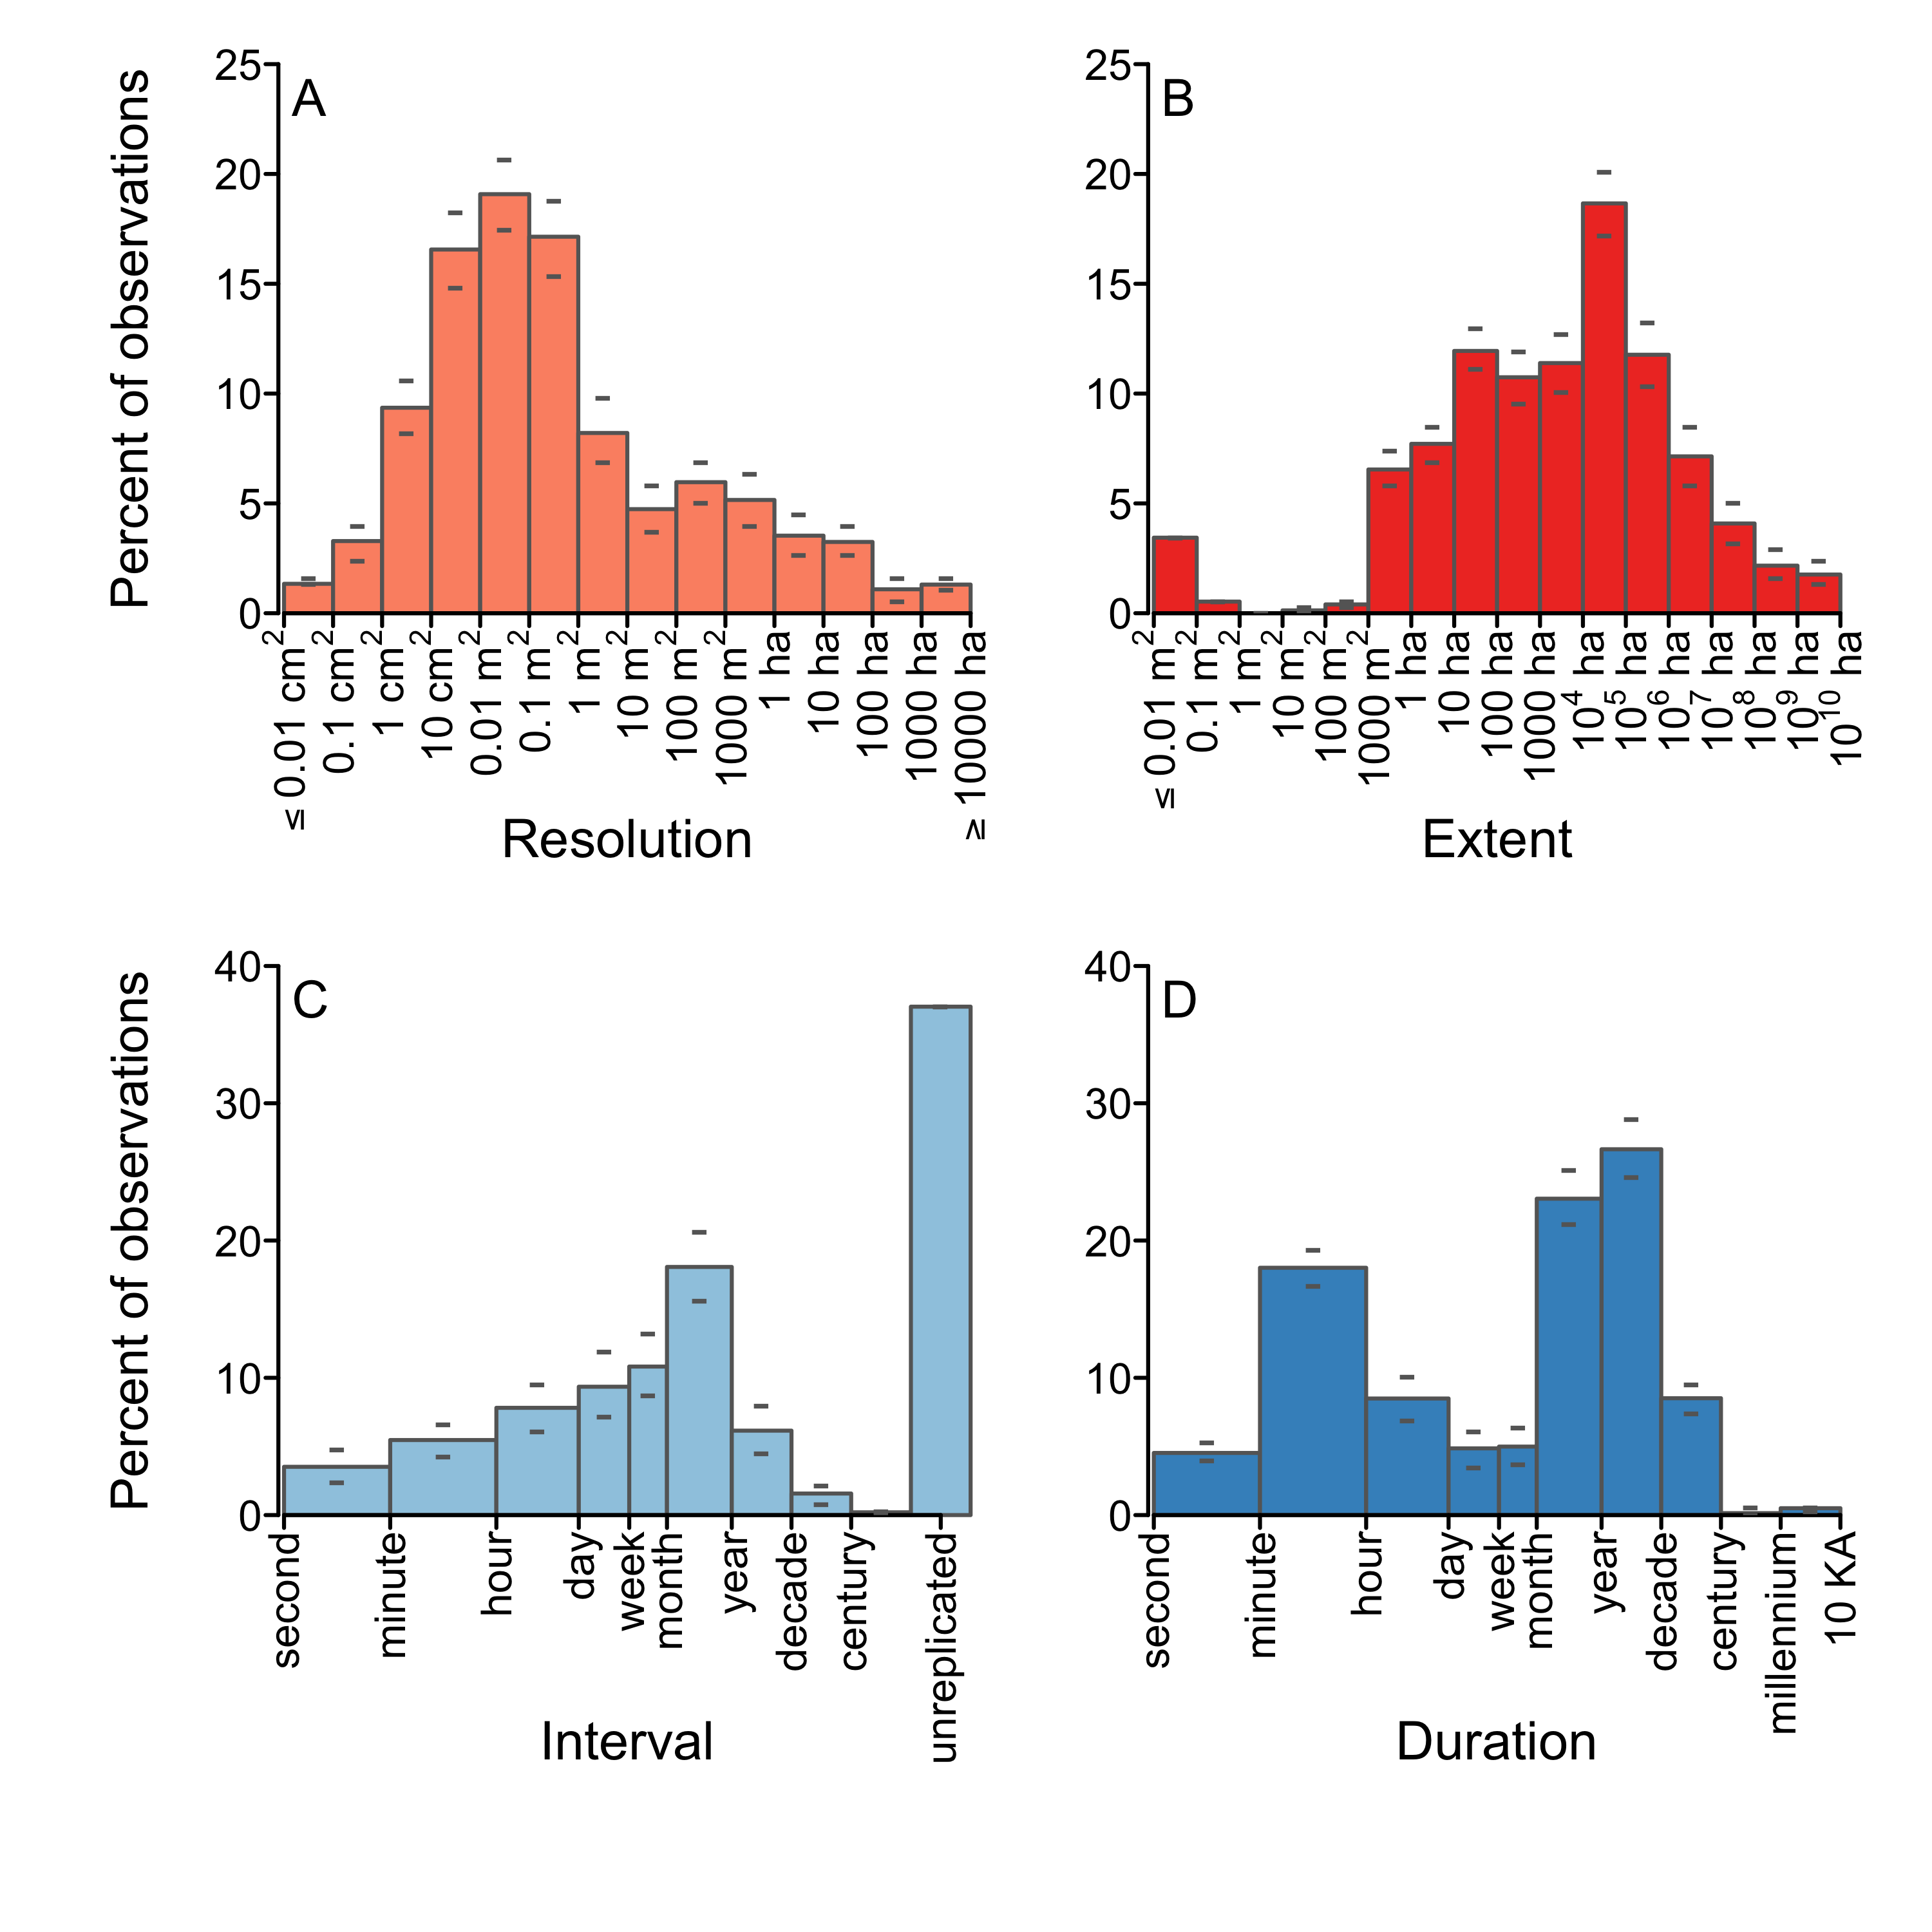
\includegraphics[width=1\textwidth]{../vignettes/figures/fig1.png}
\vspace{-0.15 cm}
\caption{Histograms of the resolution (A), extent (B), interval (C), and duration (D) of observations collected from the surveyed ecological studies. Bars represent the average percentages for each bin realized after 1000 perturbed resamples, while grey bars indicate the 95\% confidence interval. Bar widths in C-D indicate differences in scale between x-axis labels. The grey vertical line in D indicates that the majority ($>$95\%) of observations of $\leq$1 day duration were temporally unreplicated.}
\label{afoto1}
\end{figure}


\begin{figure}[!ht]
%\begin{wrapfigure}{c}{1\textwidth}
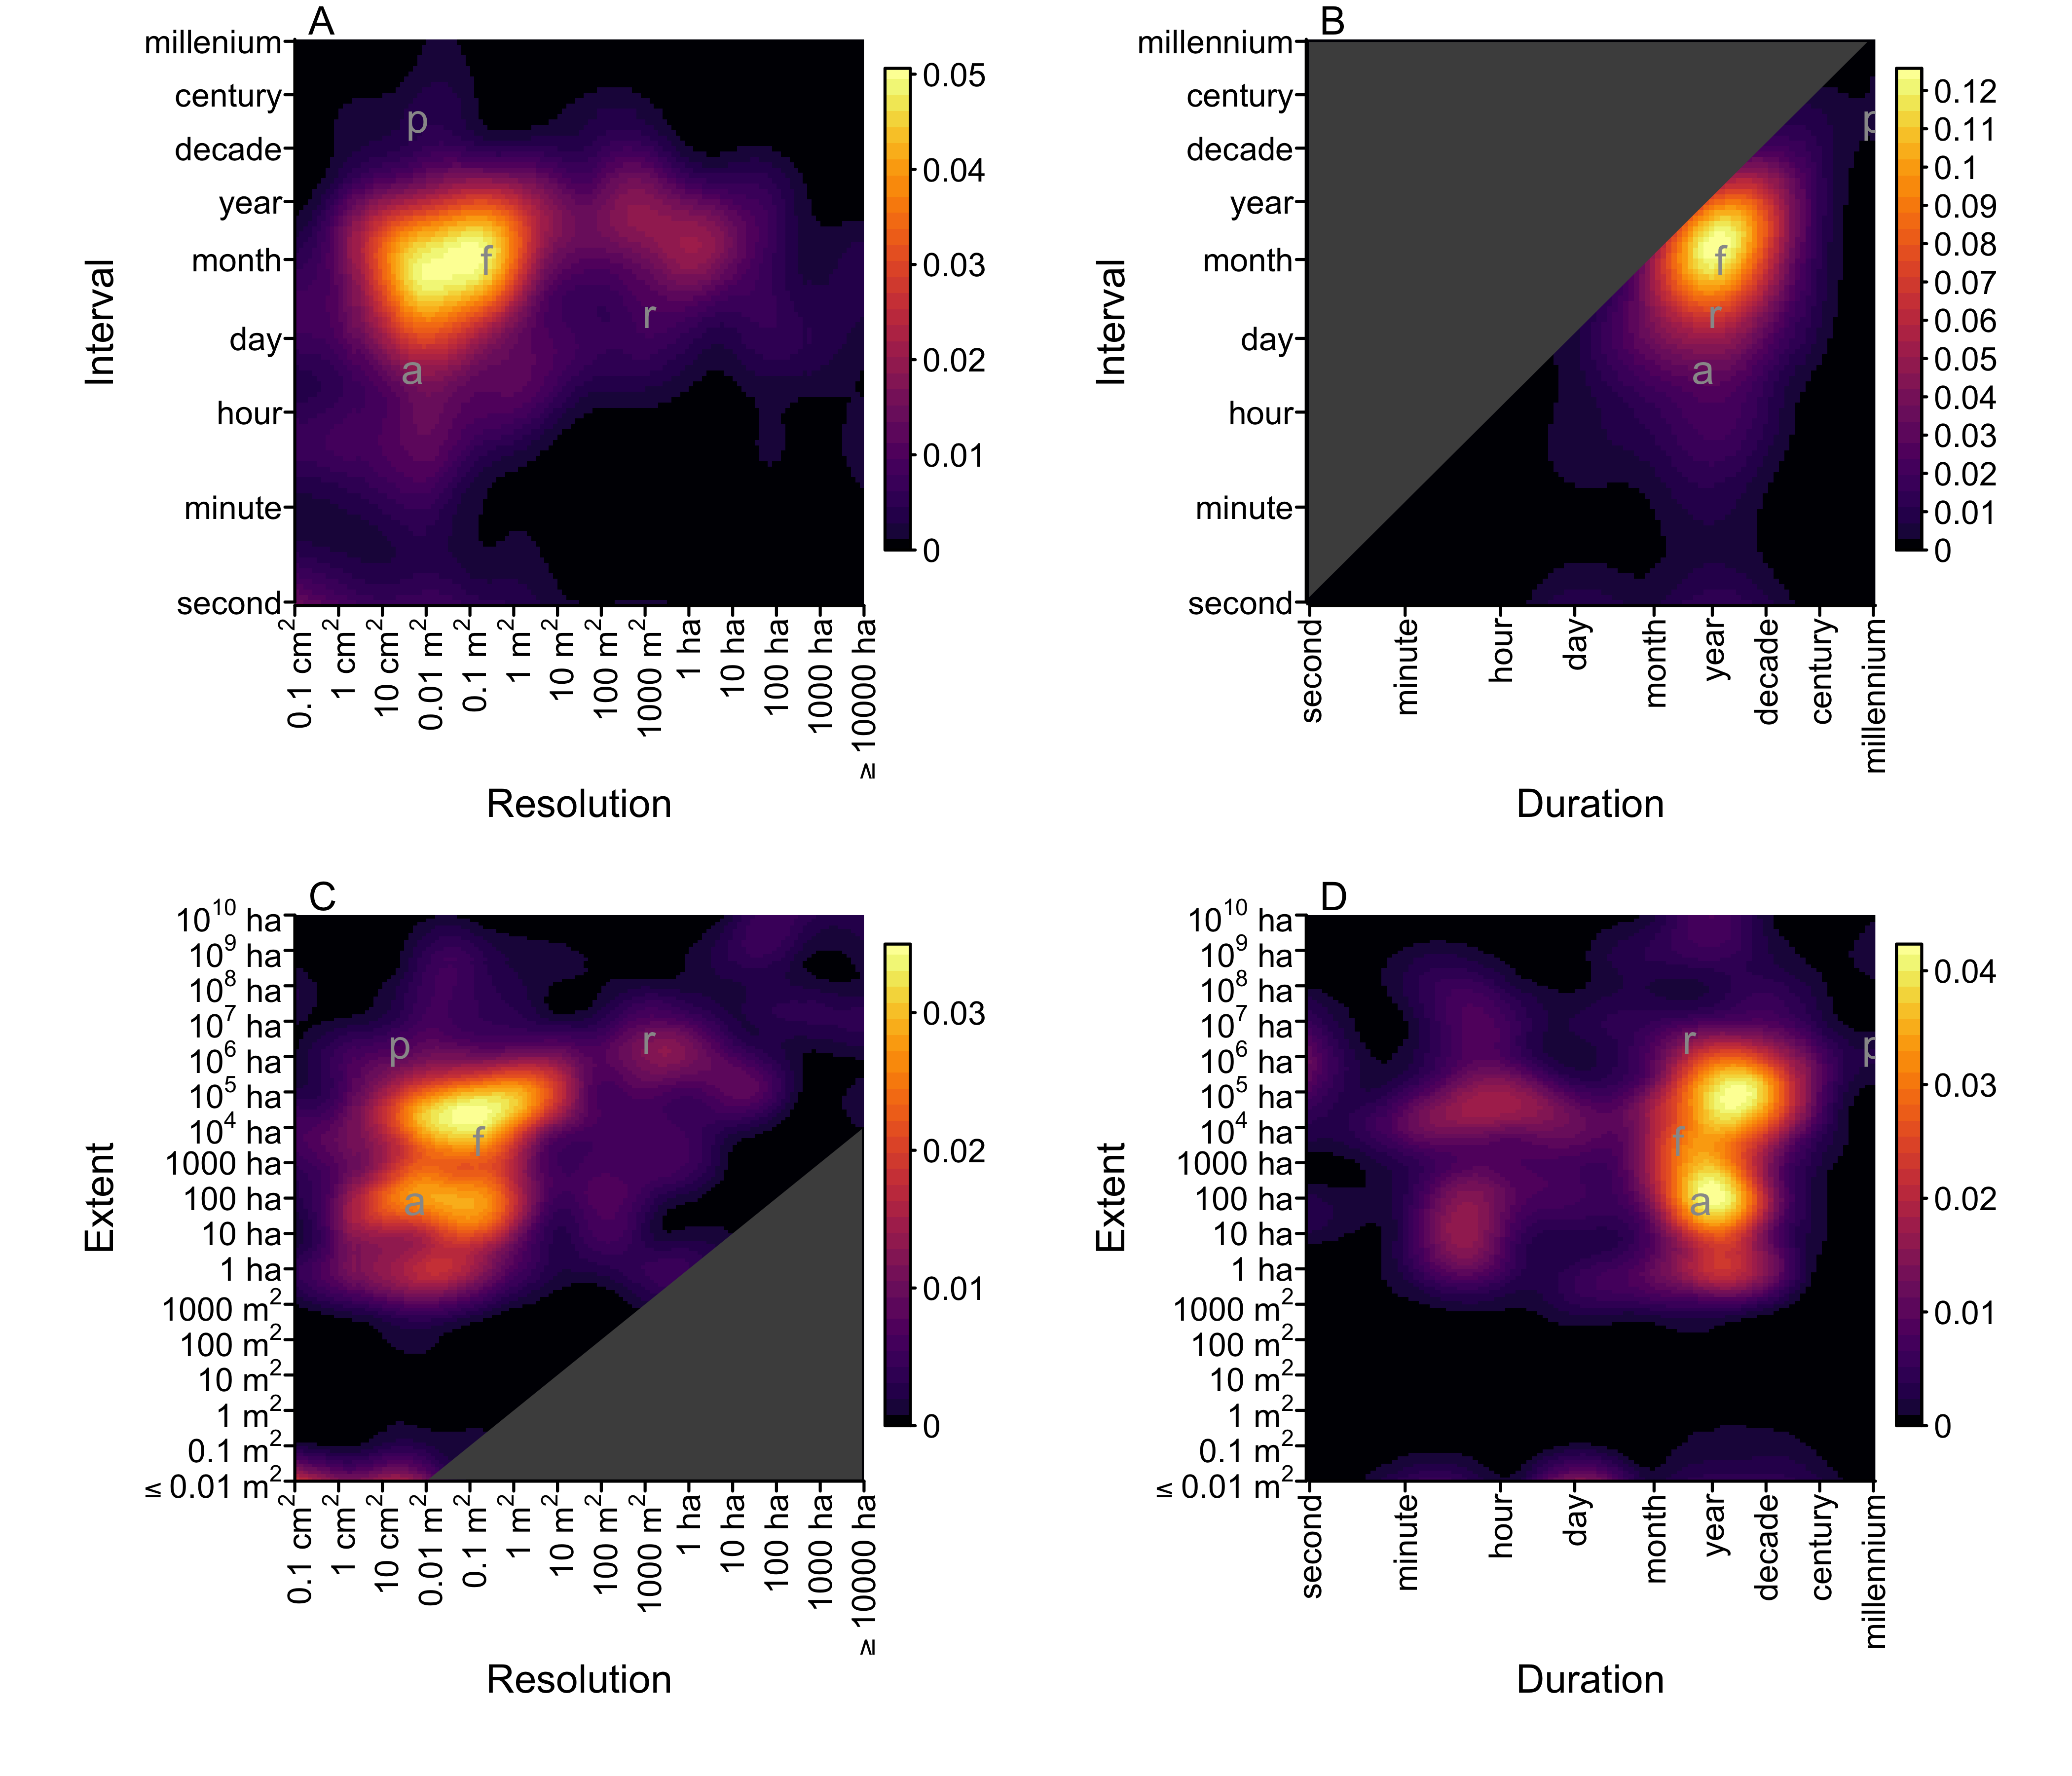
\includegraphics[width=1\textwidth]{../vignettes/figures/fig2.png}
\vspace{-0.15 cm}
\caption{Kernel density estimates of observational densities within the domains defined by A) interval and resolution (of temporally replicated observations only), B) duration and extent, C) resolution and extent, and D) interval and duration (of temporally replicated observations). Density estimates were applied to the log-transformed values of each observational dimension, and density estimates are rescaled to represent percentages. Letters in the plots denote the median values of different observational methods (f=field observations; a = automated sensing; r = remote sensing; p = paleo-observations). The grey shaded areas represent physically impossible domains (intervals greater than duration and resolutions greater than extent). Density values below the lower 3rd percentile fall within the darkest portion of the color gradient.}
\label{afoto1}
\end{figure}

\begin{figure}[ht]
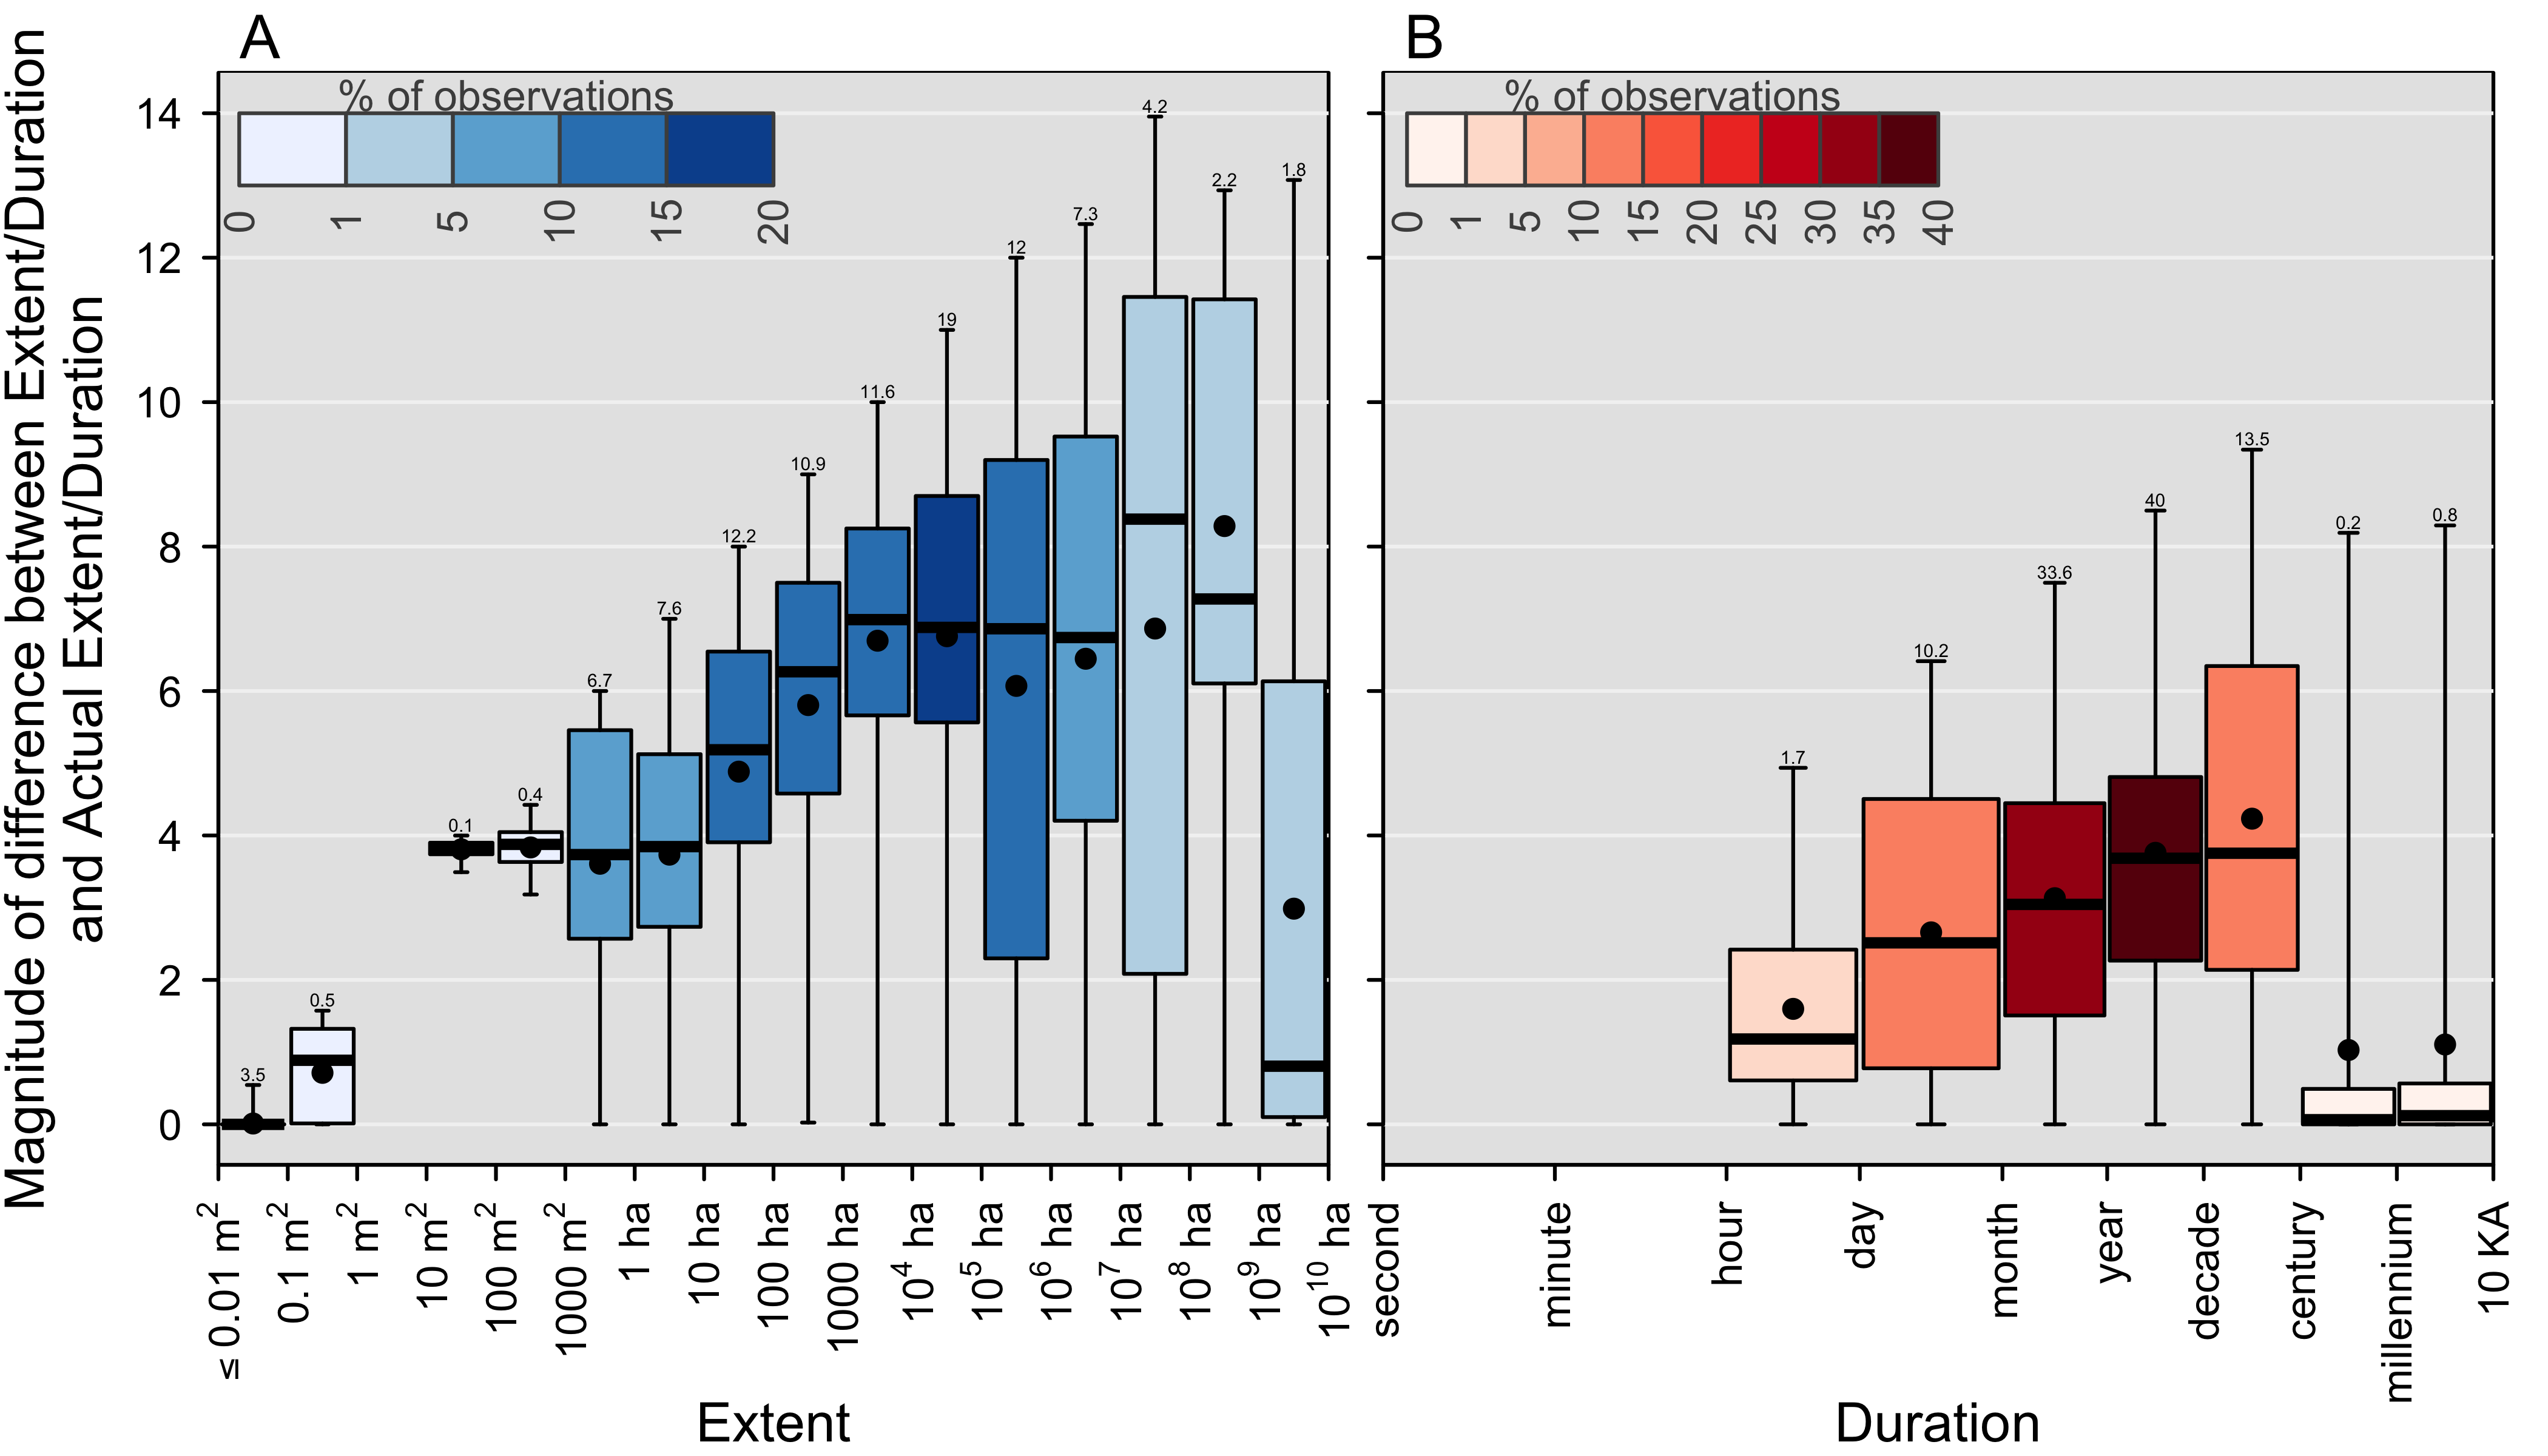
\includegraphics[width=1\textwidth]{../vignettes/figures/fig3.png}
\vspace{-0.2 cm}
\caption{The difference between extent and \emph{actual} extent (the summed area of spatial replicates) (A) and duration and \emph{actual} duration (the summed sampling duration across temporal replicates) (B). Difference values are expressed in terms of how many orders of magnitude larger (or longer) extent (duration) is than actual extent (actual duration), and are summarized (as box plots, with circle in box representing the mean and line the median) in bins representing increasing scales of actual extent/duration.  The percentages of observations falling within each bin are indicated by the color of the inter-quartile and the numeric value above the upper whisker. The grey vertical line in D indicates that the majority ($>$95\%) of observations of $\leq$1 day duration were temporally unreplicated.}
\label{afoto1}
\end{figure}


\end{document}




















